\section{Introduction}

\begin{frame}{Introduction}
    \begin{itemize}
        \item \alert{Digital transformation} is a thorough transformation of business through digital technologies.
        \item Critical in this process: accurately describing the business process to be digitised.
        \item This paper introduces agent-based simulation models for richer feedback in the transformation process.
    \end{itemize}
\end{frame}

\begin{frame}{Problem Definition}
    \begin{itemize}
        \item Traditional token-based simulations provide limited feedback for business process transformations.
        \item Proposal: Integrate ontology-based agent models into intelligent virtual environments (IVE).
        \item The addition of gamification can enhance feedback quality by simulating more nuanced, real-world interactions.
    \end{itemize}
\end{frame}

\begin{frame}{Related Work}
    \begin{multicols}{2}
        \begin{itemize}
            \item \alert{Intelligent Agents}: Systems capable of perceiving and acting upon their environment.
            \item \alert{Intelligent Virtual Environments (IVE)}: Combine high-fidelity environmental simulations with AI for real-time interaction.
            \item \alert{Digital Twins}: Real-time synchronizations between virtual and physical systems.
        \end{itemize}

        \columnbreak

        \centering
        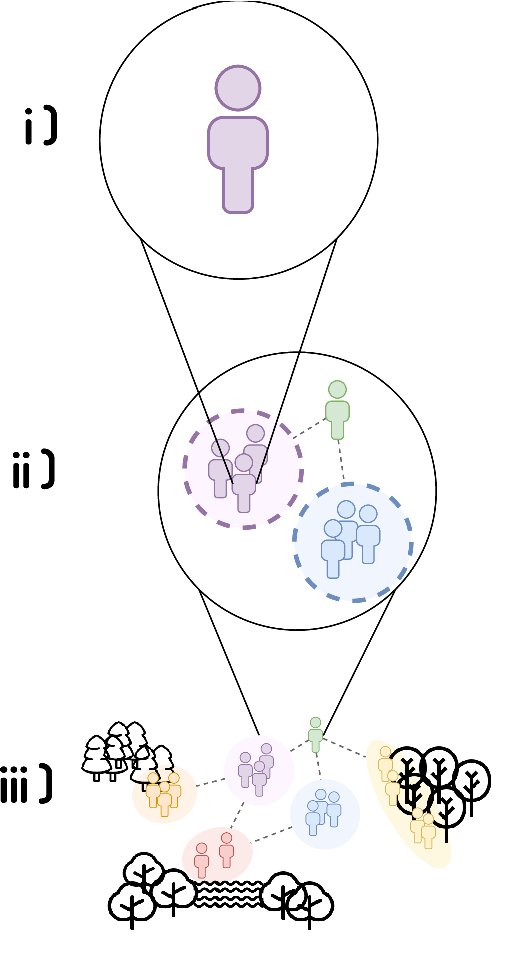
\includegraphics[width=0.5\linewidth]{Documents/240918 CECIIS @ UNIZG FOI/Figures/Agent_MAS_IVE.pdf}
    \end{multicols}
\end{frame}

\section{Proposed Architecture}

\begin{frame}{Proposed Architecture}
    \begin{itemize}
        \item Three-phase architecture:
        \begin{itemize}
            \item \alert{Setup phase}: Map real-world elements to the virtual environment using an ontology.
            \item \alert{Implementation phase}: Translate ontology-based models into simulation-ready blueprints.
            \item \alert{Execution phase}: Use data to simulate agent behaviours and observe feedback.
        \end{itemize}
        \item Agents are implemented as digital twins, and their behaviour is observed using different levels of integration.
    \end{itemize}
\end{frame}

\begin{frame}{Proposed Architecture}
    \centering
    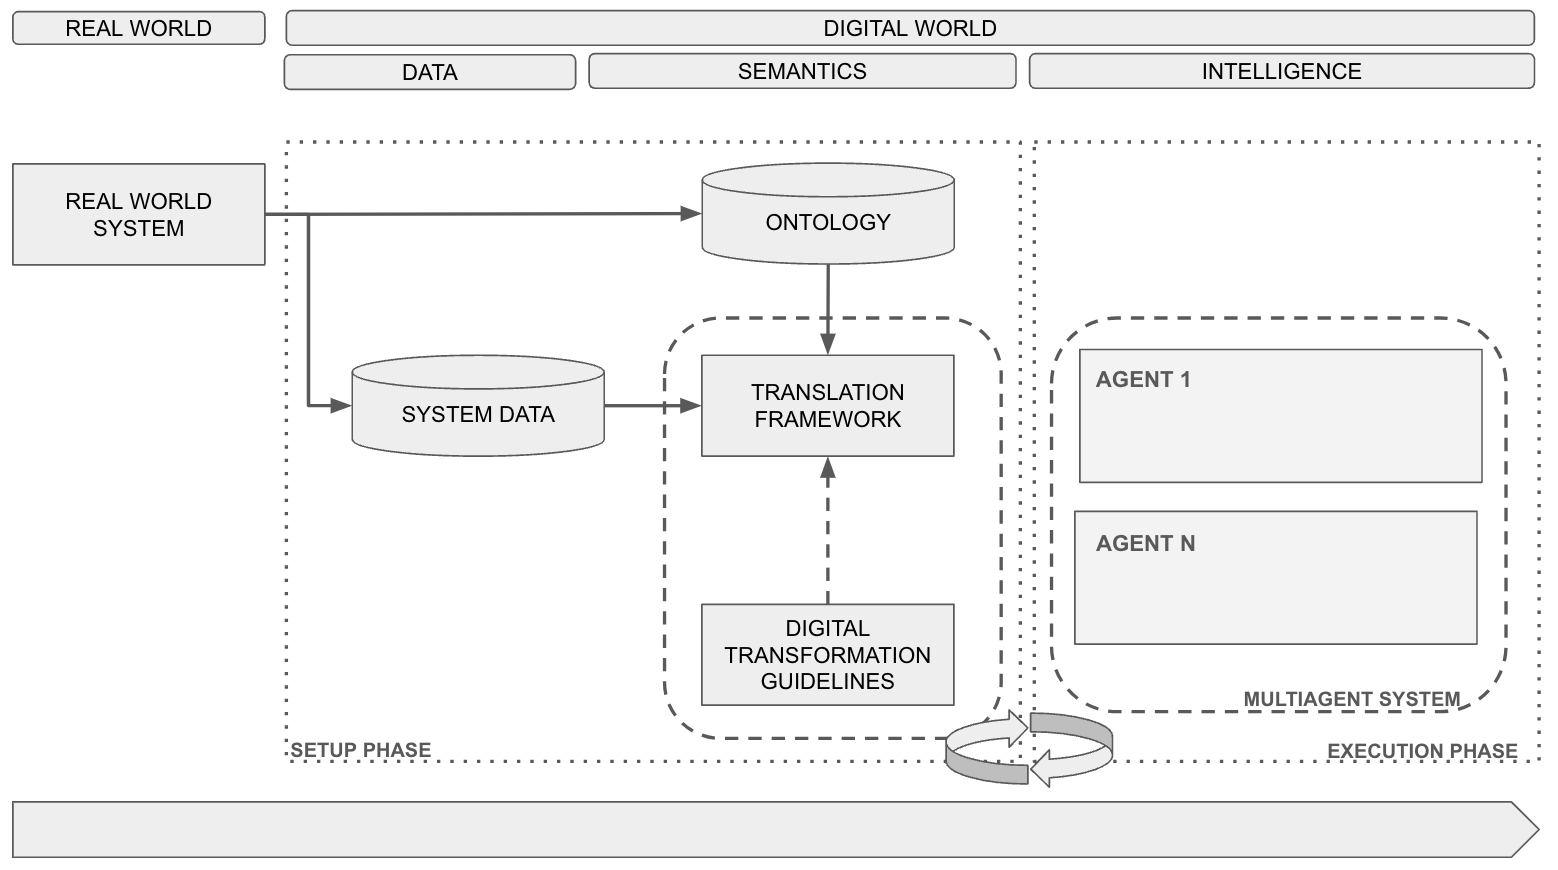
\includegraphics[width=0.8\linewidth]{Documents/240918 CECIIS @ UNIZG FOI/Figures/CECIIS-DT-ARCHITECTURE-II.png}
\end{frame}

\section{Use Cases}

\begin{frame}{Use Case: Production Planning}
    \begin{itemize}
        \item Production planning and scheduling process
        \item The proposed architecture simulates the impact of digital transformation in these phases.
    \end{itemize}

    \centering
    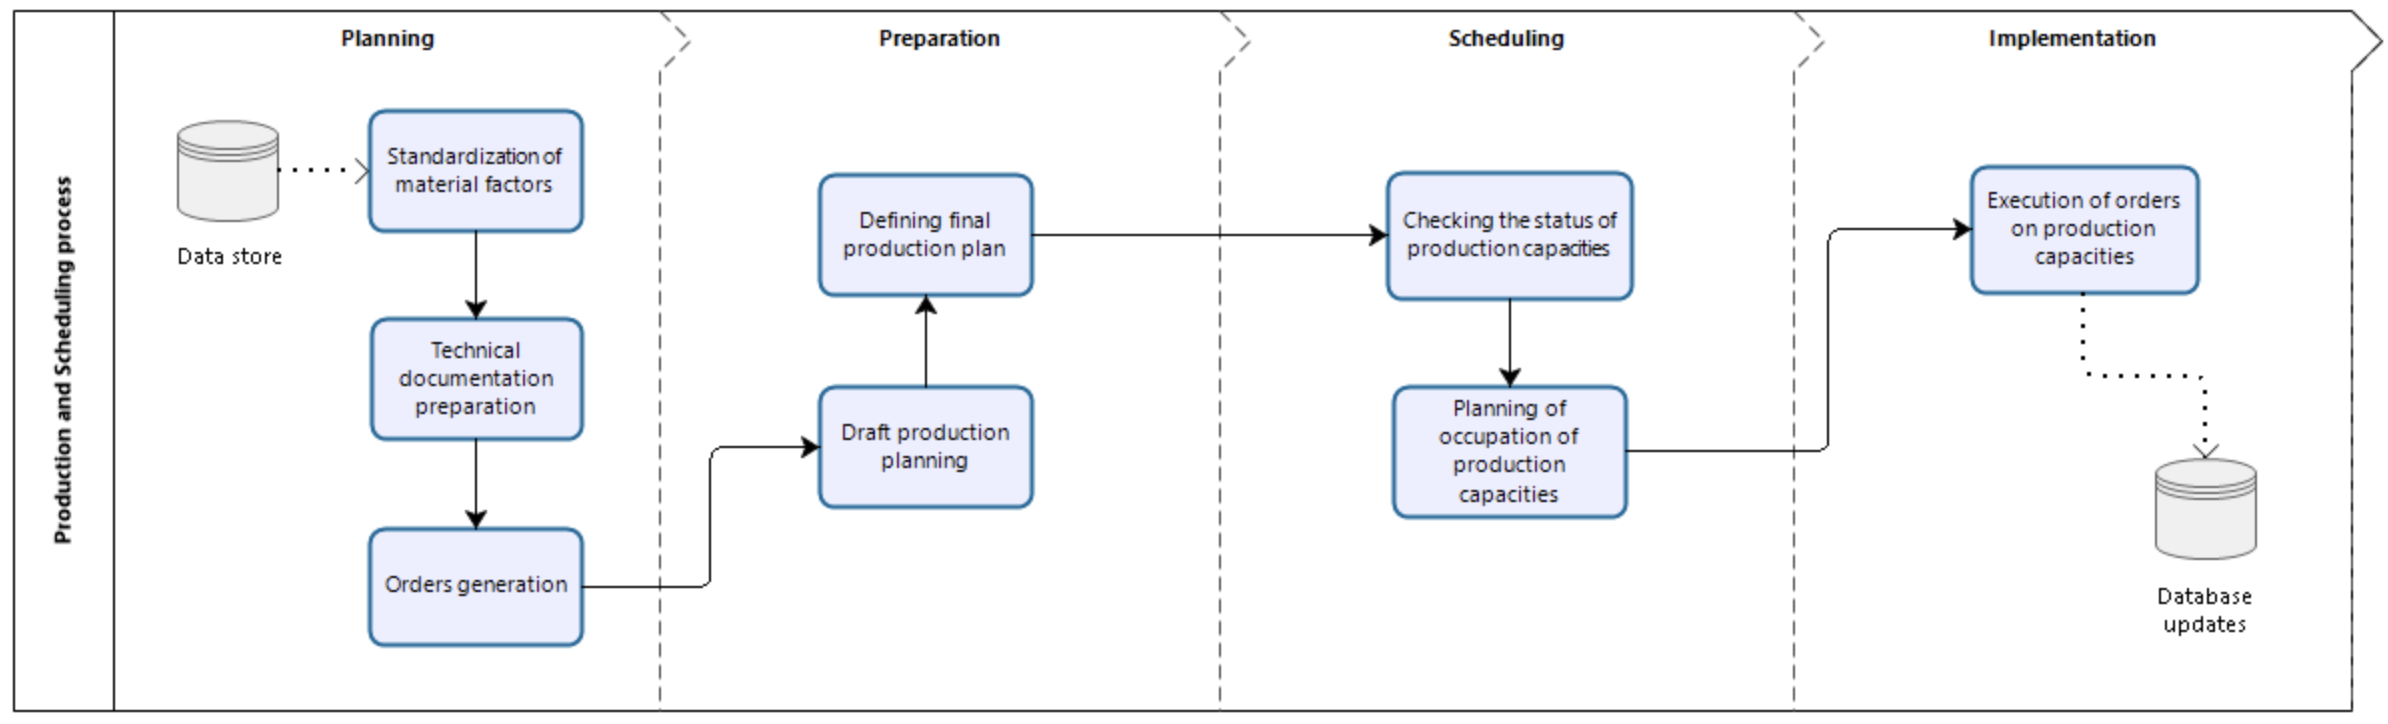
\includegraphics[width=0.9\linewidth]{Documents/240918 CECIIS @ UNIZG FOI/Figures/CECIIS-USE-CASE-PHASES.png}
\end{frame}

\begin{frame}{Scenario 1: Planning and Preparation}
    \begin{itemize}
        \item Digital inputs (material stocks, work orders) are synchronized in real-time.
        \item Production plans dynamically adjust to changes in the market and inventory.
        \item Simulation models customer orders, inventory, and suppliers as interacting agents.
    \end{itemize}
\end{frame}

\begin{frame}{Scenario 2: Scheduling and Implementation}
    \begin{itemize}
        \item Work orders are allocated digitally to available resources.
        \item Real-time updates provide continuous feedback on capacity and workload.
        \item Simulation adjusts production plans based on incidents like equipment failures.
    \end{itemize}
\end{frame}

\section{Discussion and Conclusion}

\begin{frame}{Discussion}
    \begin{itemize}
        \item Simulating digital transformation using agents offers richer, more interactive feedback than traditional methods.
        \item Incorporating gamification techniques mimics real-world human behavior changes.
        \item Applications of AI in business process modeling create more accurate transformation insights.
    \end{itemize}
\end{frame}

\begin{frame}{Conclusion and Future Work}
    \begin{itemize}
        \item Contributions: A three-phase simulation framework using agents, ontologies, and gamification.
        \item Future Research:
        \begin{itemize}
            \item Expanding ontology for business processes.
            \item Integrating machine learning for more advanced decision-making.
            \item Validating the framework with empirical case studies.
        \end{itemize}
    \end{itemize}
\end{frame}
